%\subsection{Histogramm f\"ur Input Data (153)}
%\begin{figure}
\begin{center}
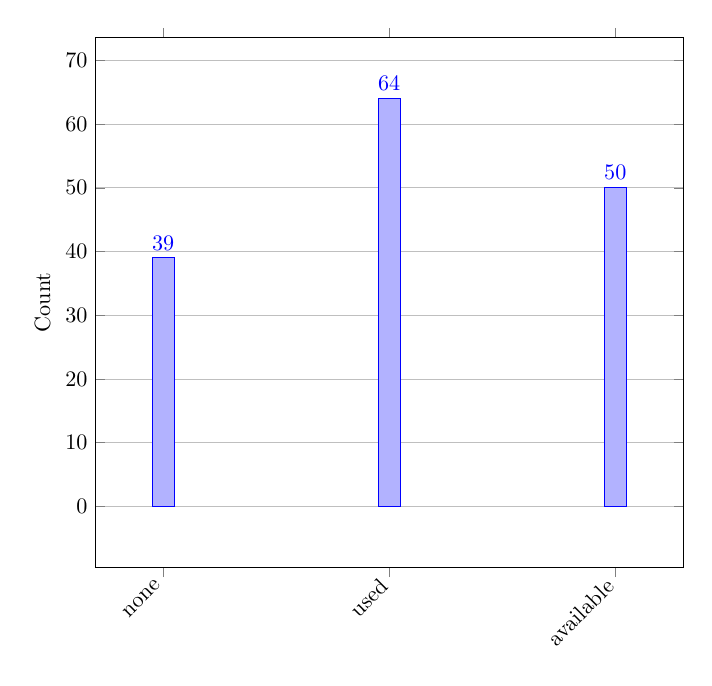
\begin{tikzpicture}[scale=.8]
\begin{axis}[ ybar, ymajorgrids, enlargelimits=0.15, legend style={at={(0.5,-0.15)}, anchor=north,legend columns=-1},
    width=.90\linewidth,height=10cm,
    nodes near coords, %nodes near coords align=below,
    ylabel={Count}, ymin=0,
    x tick label style={rotate=45,anchor=east},
    xtick={1,2,3},
    xticklabels={none,used,available
}
    %xlabel={Input Data}    
    ]
  \addplot coordinates { (1,39)  (2,64)  (3,50)   };
\end{axis}
\end{tikzpicture}
\end{center}
%\caption{Histogramm f\"ur Input Data (153)}
%\label{fig:histo_inputdata}
%\end{figure}

